\subsection{Знакопеременные ряды}
\begin{definition}
    Если для ряда
    \[\sum_{n=1}^{\infty}a_n \eqno{(1)}\]
    ряд
    \[\sum_{n=1}^{\infty}|a_n|\]
    сходится, то ряд (1) называется абсолютно сходящимся.
\end{definition}
\begin{statement}
    Если ряд
    \[\sum_{n=1}^{\infty}a_n\]
    абсолютно сходится, то он сходится.
\end{statement}
\begin{proof}
    По критерию Коши:
    \[\left|\ \sum_{n=k}^{N}a_n\ \right|\leq \sum_{n=k}^{N}|a_n|<\epsilon\]
\end{proof}
\begin{definition}
    Биекция $\sigma: \N\to \N$ называется перестановкой натурального ряда.
\end{definition}
\begin{theorem}
    Если ряд
    \[\sum_{n=1}^{\infty}a_n \eqno{(1)}\]
    абсолютно сходится, то для любой перестановки $\sigma$ натурального ряда, ряд
    \[\sum_{n=1}^{\infty}a_{\sigma(n)} \eqno{(2)}\]
    абсолютно сходится и их суммы равны.
\end{theorem}
\begin{proof}
    Пусть $a_n\geq 0$. Рассмотрим
    \[S_k^{\sigma}=\sum_{n=1}^{k}a_{\sigma(n)}\]
    Пусть $N=\max\limits_{1\leq n\leq k}{\sigma(n)},\ S_n\to S$. Тогда
    \[S_k^{\sigma}\leq S_N \Rightarrow S_k^{\sigma}\leq S \Rightarrow \exists\ S^{\sigma}=\lim\limits_{k\to \infty}S_k^{\sigma}\]
    Используя, что (2) абсолютно сходится, аналогично, поменяв ряды местами, получим:
    \[S\leq S^{\sigma} \Rightarrow S=S^{\sigma}\]
    тогда
    \[\sum_{n=1}^{\infty}|a_n|=\sum_{n=1}^{\infty}|a_{\sigma(n)}|\]
    заметим, что
    \[a+|a|=\begin{cases}
        2a,\ a\geq 0,\\
        0,\ a<0.
    \end{cases}\]
    значит
    \[\sum_{n=1}^{\infty}(a_n+|a_n|)=\sum_{n=1}^{\infty}(a_{\sigma(n)}+|a_{\sigma(n)}|)\]
    отсюда
    \[\sum_{n=1}^{\infty}a_n=\sum_{n=1}^{\infty}a_{\sigma(n)}\]
\end{proof}
\begin{definition}
    Рассмотрим ряды
    \[\sum_{n=1}^{\infty}a_n,\ \sum_{n=1}^{\infty}b_n\]
    а также всевозможные попарные произведения
    \[\{a_n\cdot b_k\}_{n=1,k=1}^{\infty,\ \ \infty}\]
    Будем записывать ряд по схеме:

    \begin{center}
        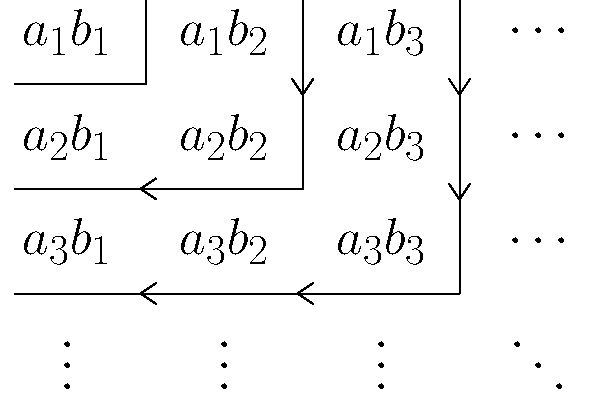
\includegraphics[width=6cm]{Images/image-1.pdf}
    \end{center}
    % \[\begin{matrix}
    %     a_1b_1 & a_1b_2 & a_1b_3 & \dots\\
    %     a_2b_1 & a_2b_2 & a_2b_3 & \dots\\
    %     a_3b_1 & a_3b_2 & a_3b_3 & \dots\\
    %     \vdots & \vdots & \vdots
    % \end{matrix} \eqno(*)\]
    То есть, запишем в порядке: 
    \[a_1b_1,\ a_1b_2,\ a_2b_2,\ a_2b_1,\ a_1b_3,\ a_2b_3,\ a_3b_3,\ a_3b_2,\ a_3b_1,\ \dots\]
    Тогда ряд:
    \[\sum_{m=1}^{\infty}(a_nb_k)_m\]
    называется произведением рядов по прямоугольной схеме ($*$).
\end{definition}
\begin{statement}
    Пусть два ряда
    \[\sum_{n=1}^{\infty}a_n=A,\ \sum_{n=1}^{\infty}b_n=B\]
    сходятся абсолютно. Тогда
    \[\sum_{m=1}^{\infty}(a_n b_k)_m \eqno{(*)}\]
    сходится абсолютно и равен $AB$.
\end{statement}
\begin{proof}
    Рассмотрим подпоследовательность частичных сумм ряда ($*$), которые имеют вид $S_{N^2}$:
    \[S_{N^2}=S_N^a\cdot S_N^b \Rightarrow S_{N^2} \to AB,\ N\to \infty\]
    Теперь перейдем к общему виду $S_{N^2+M},\ (1\leq M\leq 2N)$ и покажем, что вклад членов, добавляемых к квадратной частичной сумме, бесконечно мал
    \[S_{N^2+M}=S_{N^2}+\sum_{m=N^2+1}^{N^2+M}(a_n\cdot b_k)_m\]
    обозначим
    \[S_{N,M}=S_{N^2+M}-S_{N^2}=\sum_{m=N^2+1}^{N^2+M}(a_n\cdot b_k)_m\]
    \[|S_{N,M}|\leq |b_{N+1}|\cdot(|a_1|+\dots+|a_{N+1}|)+|a_{N+1}|\cdot (|b_1|+\dots+|b_N|)\to 0\]
    поскольку частичные суммы каждого ряда ограничены и члены, по необходимому признаку, стремятся к нулю. Значит $S_{N^2+M}\to AB$.
    % пояснить почему ряд сходится абсолютно!!!!!!!
\end{proof}
\begin{definition}
    Если ряд
    \[\sum_{n=1}^{\infty}a_n \eqno{(*)}\]
    сходится, а ряд
    \[\sum_{n=1}^{\infty}|a_n|\]
    расходится, то ряд ($*$) называется условно сходящимся.
\end{definition}
\begin{statement}
    Пусть ряд
    \[\sum_{n=1}^{\infty}a_n\]
    условно сходится. Обозначим
    \[a_n^+\begin{cases}
        a_n,\ a_n>0,\\
        0,\ a_n\leq 0.
    \end{cases},\ a_n^-=\begin{cases}
        0,\ a_n\geq 0,\\
        a_n,\ a_n<0.
    \end{cases}\]
    Тогда ряды
    \[\sum_{n=1}^{\infty}a_n^+ \eqno(1)\]
    \[\sum_{n=1}^{\infty}a_n^- \eqno(2)\]
    расходятся к $+\infty$ и $-\infty$ соответственно.
\end{statement}
\begin{proof}
    Если оба ряда сходятся, то
    \[\sum_{n=1}^{\infty}|a_n|=\sum_{n=1}^{\infty}a_n^+-\sum_{n=1}^{\infty}a_n^-\]
    сходится, противоречие.
    Если ряд (1) сходится, а (2) расходится, то
    \[\sum_{n=1}^{\infty}a_n^-=\sum_{n=1}^{\infty}a_n-\sum_{n=1}^{\infty}a_n^+\]
    сходится, противоречие. Аналогичное противоречие в случае, когда $(2)$ сходится, а $(1)$ расходится. Значит оба ряда расходятся.
\end{proof}
\begin{theorem} (Теорема Римана)\\
    Если ряд
    \[\sum_{n=1}^{\infty}a_n\]
    сходится условно, то $\forall a\in \R\ \exists\ \sigma_a$ такая, что
    \[\sum_{n=1}^{\infty}a_{\sigma_a(n)}=a\]
    $\exists\ \sigma_{\pm \infty}$ такая, что
    \[\sum_{n=1}^{\infty}a_{\sigma_{\pm \infty}}=\pm \infty\]
    $\exists\ \sigma$ такая, что
    \[\sum_{n=1}^{\infty}a_{\sigma(n)}\]
    расходится, но частичные суммы ограничены.
\end{theorem}
\begin{proof}
    доказали картинками)))))\\
    \textit{доказательство появится немного позже}
\end{proof}